%\newpage
\vspace{-0.25cm}

\subsection{Performance Issues with Self-Hosting on JIT Compilers}
\label{subsec:performance}

With many micro and macro benchmarks and larger experiments, the
existing Pycket implementation is shown to be significantly performant
in evaluating Racket code. It benefits from the the existing generic
optimizations in the RPython framework, including common subexpression
elimination, copy propogation, constant folding, loop invariant code
motion, malloc-removal and the inlining that naturally comes for free
from tracing \cite{loop-aware:12, hotpath:06, malloc-removal:11}, as
well as from many improvements on the interpreter such as environment
pruning, data structure specialization, strategies, as well as some
gradual typing related improvements such as the use of
hidden-classes. However, it is also shown that in some cases Pycket is
significantly slower than all the other systems, on "almost
exclusively recursive programs with data-dependent control flow in the
style of an interpreter over an AST" \cite{pycket15, pycket17}. In
this section we identify the key points of these issues and propose
solution approaches that will be essential in implementing efficient
run-times for self-hosting functional langauges on meta-tracing JIT
compilers.

\begin{figure}[h!]
  %\vspace{-0.5cm}
  \footnotesize
  \begin{mdframed}
\begin{lstlisting}[mathescape,escapechar=\%,language=lisp]
a 	Matches the specified character literal          q       q
* 	Matches 0 or more of the previous character      a*      "", a, aa, aaa
. 	Matches any character literal                    .       a, b, c, d, e ...
^ 	Matches the start of a string                    ^c      c, ca, caa, cbb ...

(define (match-star pattern p-pos str s-pos star-pos m)
  (or (and (< s-pos (string-length str)) (char=? (string-ref pattern p-pos) (string-ref str s-pos))
            (%\underline{match-pat}% pattern p-pos str (add1 s-pos) (cons (string-ref str s-pos) m)))
       (%\underline{match-pat}% pattern (add1 star-pos) str s-pos m)))

(define (match-pat pattern p-pos str s-pos m)
  (cond
    [(>= p-pos (string-length pattern)) m]
    [(and (< (+ p-pos 1) (string-length pattern)) (char=? (string-ref pattern (+ p-pos 1)) #\*))
      (%\underline{match-star}% pattern p-pos str s-pos (+ p-pos 1) m)]
    [(char=? (string-ref pattern p-pos) #\.)
      (and (< s-pos (string-length str)) (%\underline{match-pat}% pattern (add1 p-pos) str (add1 s-pos) (cons (string-ref str s-pos) m)))]
    [else
     (and (char=? (string-ref pattern p-pos) (string-ref str s-pos))
           (%\underline{match-pat}% pattern (add1 p-pos) str (add1 s-pos) (cons (string-ref str s-pos) m)))]))

(define (reg-match pattern str)
  (let ([m (cond
             [(char=? (string-ref pattern 0) #\^) (match-pat pattern 1 str 0 '())]
             [(string=? str "") (match-pat pattern 0 str 0 '())] ; edge case
             [else (for/or ([i (in-range (string-length str))])
               (match-pat pattern 0 str i '()))])])
    (and m (list (list->string (reverse m))))))
\end{lstlisting}
\end{mdframed}
\caption{A simple regular expression matcher (some cases are removed for space).}
\label{fig:regexp}
\vspace{-0.3cm}
\end{figure}

Tracing interpreter-style programs with complex control-flow paths is
a known weakness of JIT compilers. The large number of indirections
not only cripple the JIT optimizations but also causes the loops to be
segmented into a large number of highly data driven traces. For
example, consider the following program in \figref{fig:regexp}, which
is a very simple regular expression matcher. It is highly simplified
and some of the rules are removed for space.

%

Tracing this program running with an input regexp, say
$\mathtt{\#}$\racketcode{rx"defg"}, trying to match it against an
input string produces a trace that follows the control-flow path of
the program for that input, making tracing quite wasteful because for
any other input regexp, say $\mathtt{\#}$\racketcode{rx"a*"} which
follows an entirely different path on the program, the JIT produces,
compiles and optimizes yet another trace for that input, unable to use
the previously generated trace. This problem not only increases the
warmup time but also produces traces that are unlikely to be
frequently re-used.

This problem is immediately observable on Pycket self-hosting Racket
through the expander linklet, because the interpreter style programs
with complex control-flow paths are quite central in self-hosting a
language (e.g. expand, fasl etc.). Additionally, since the Pycket's
level of language abstraction is increased one step further, the
generated traces are much larger, which creates a pressure for the
JIT's compiler and optimizer. As a result, in the run-time the JIT
spends a lot of time compiling and optimizing traces, but often bails
out and interprets the code instead of using the traces, which defeats
the purpose of using a tracing JIT.

%% The major part of the problem is about loop-detection. While the loop
%% detection is in general quite central in tracing JITs, for Pycket it
%% is a bit more tricky, as Pycket works on a higher level of abstraction
%% (program AST) than a lower-level bytecode interpreter, and the only
%% way to create a loop is through a function application. Moreover, the
%% self-hosting adds yet another level of abstraction on top, making the
%% loop detection in the source-level even more difficult.

Another major actor in this play is the loop invariant code motion
optimization performed by the JIT \cite{loop-aware:12}. This
optimization prepends a trace to itself, moving all the loop-invariant
operations (usually the operations for destructuring the interpreter
state) into the preamble, keeping all the essential operations in the
peeled-iteration (the inner loop). An example of this can be seen in
the trace in \figref{fig:trace} in \secref{subsec:rpython}. Any trace
or a side-trace (i.e. a \emph{bridge}) that is able to jump to the
peeled-iteration of another trace therefore saves time by not
performing the loop-invariant operations. In order to do so, however,
the program state needs to be consistent with the one that is expected
by the peeled-iteration.

The program state consists of heap allocated objects
(e.g. environment, continuation), the virtuals (malloc-removed parts
of the interpreter state), and other loop information such as range
values. In order to jump to a peeled-iteration, the state needs to
match with the one that the iteration is expecting, e.g. the same
state at the end of its preamble. On the other hand, jumping to the
preamble of a trace requires the allocation of all the unallocated
parts of the interpreter state. If a bridge for a side-exit is used to
jump back to the original trace, the JIT tries to make it jump to the
peeled-iteration whenever possible to avoid performing the
loop-invariant operations. However, this often fails on Pycket because
the interpreter state often can't match the expected state, because
the state is changed differently by different control flow paths
(e.g. non-tail calls add a continuation frame). Note that in Pycket
the major part of the interpreter state is the environment and the
continuation, which are heap allocated objects.

This issue is partly addressed in the previous versions of Pycket by
allowing the JIT to allocate a little bit more to force a match
between the states. The malloc-removal and escape analysis in the
trace optimizer often allows the JIT to remove parts of state and
create virtuals for the objects that never escape the loop
\cite{malloc-removal:11, loop-aware:12}. The introduced heuristic on
Pycket allows the JIT to allocate such objects elided by the
optimizations, trading some space for jumping into the inner loop to
avoid performing loop-invariant operations. It is shown that with this
heuristic the performance in gradual typing is increased by 4\% on
Pycket, while adding no extra overhead \cite{pycket17}.

\begin{wrapfigure}[26]{r}{0.40\textwidth}
    %\vspace{-0.5cm}
    \centering
    \begin{minipage}[t]{0.38\textwidth}
      \begin{minted}[numbersep=0pt,gobble=0,linenos,numbers=right,fontsize=\scriptsize,frame=lines]{python}
# start of the trace (preamble)
label(i0, p1, descr="124248176")
i3 = int_add(i0, 1)
p4 = getfield_gc_r(p1, descr="StrMatchContext.string")
i5 = strgetitem(p4, i0)
i7 = int_eq(i5, 100)
guard_false(i7)
i8 = getfield_gc_i(p1, descr="FixedMatchContext.end")
i9 = int_lt(i3, i8)
guard_true(i9)
# peeled-iteration (inner loop)
label(i3, p1, p4, i8, descr="124248256")
i11 = int_add(i3, 1)
i12 = strgetitem(p4, i3)
i14 = int_eq(i12, 100)
guard_false(i14)
i15 = int_lt(i11, i8)
guard_true(i15)
# jump
jump(i11, p1, p4, i8, descr="124248256")
    \end{minted}
    \end{minipage}
    \begin{minipage}[t]{0.38\textwidth}
      \begin{minted}[escapeinside=||,numbersep=0pt,gobble=0,linenos,numbers=right,fontsize=\scriptsize,frame=lines]{lisp}
|#|lang racket/base

(define l (make-string 4000 #\a))
(define r (make-string 4000 #\p))
(define str-big (string-append l "defg" r))

(define reg-r (regexp "defg"))

(define iter 1000000)

(time
 (for ([i (in-range iter)])
   (regexp-match reg-r str-big)))
    \end{minted}
    \end{minipage}
    \caption{\small Trace of Pycket's regexp (in RPython) matching
      $\mathtt{\#}$\racketcode{rx"defg"}}
    \label{fig:regexp-trace}
  \end{wrapfigure}

Adding the linklets layer to the front-end allows Pycket to run large
Racket programs including the expander. To give a perspective, the
offline generated expander linklet that is processed in Pycket at boot
itself is roughly 5MB file containing the s-expressions of 2642
functions. Another example is, to run a single Racket program written
in the \emph{racket/base} language (such as repl for instance), more
than 100 Racket modules need to be expanded and instantiated first
just to load the language before running the program itself. While
Pycket's performance on the micro-benchmarks is not effected by the
linklet layer (since nothing has changed in the back-end), these large
programs that are now runnable on Pycket aggravate these issues
observed before.

%% As discussed in \secref{subsec:rpython}, a trace is generated in a
%% meta-tracing framework by accompanying an interpreter while it is
%% evaluating a program and detecting hot-loops. During this process, the
%% tracer exactly follows all the operations in the interpreter. For
%% example, if a function application is being evaluated, the next
%% operation to be interpreted will be the first operation in the
%% function's body\footnote{This is why inlining comes naturally from
%%   tracing.}. While this approach works quite well in generating
%% re-usable and concise traces for programs/loops with a straightforward
%% control flow thanks to the hints and annotations in meta-tracing
%% \cite{bolz09}, it becomes significantly harder when the control flow
%% gets more complicated. Consider the following program being
%% meta-traced:

To understand the issue better, it is important to first see how the
loop detection currently works on Pycket. While for the low-level
languages such as in a bytecode interpreter a program counter is used
to detect loops, in Pycket the focus is on function applications,
since Pycket works on program ASTs and the only AST that may create
loops is an application. As reported in the previous studies, Pycket
utilizes two techniques, namely the two-state tracking and the use of
a dynamic call-graph. In both techniques the idea is to eliminate the
"false-loops" among all the observed trace headers (i.e. potential
start of a loop). The two-state tracking encodes the trace headers as
a pair of a lambda body and its call-site, and the call-graph method
detects cycles on a dynamically generated call-graph to handle extra
levels of indirection. These approaches together are proven to be very
effective in tracing code with a heavy use of shared control-flow
indirections, such as the contract system \cite{pycket15,pycket17}.

The reason that we chose the regular expression matcher as an example
in \figref{fig:regexp} is that Pycket already has an efficient regexp
implementation in RPython to compare against. As a simple experiment
to demonstrate the issue, we run both regexp implementations (the one
in the \figref{fig:regexp} and the RPython implementation) to match
$\mathtt{\#}$\racketcode{rx"defg"} against a large string containing
\racketcode{"defg"} in the middle and measure the time
performances. \figref{fig:regexp-trace} shows both the trace we get
from the RPython implementation and the program we run. To run the
simple implementation in \figref{fig:regexp}, we modify this program
to use the \racketcode{reg-match} in instead of the
\racketcode{regexp-match}. When we run both with the same inputs, we
observe 2x slowdown on the simple implementation. Part of the reason
is the use of clever techniques that are specific to the regexp
implementation on RPython such as caching and using contexts etc. The
bigger part of the problem, however, lies in the difference between
the traces that are generated for this computation.

The gist of this computation is the literal search in the string for
the \racketcode{"defg"} pattern. As can be seen in
\figref{fig:regexp-trace}, this is captured in a tight loop in the
main trace for the RPython implementation. The RPython regexp
implementation utilizes interpreter hints to control the unrolling and
encourages the allocation removal optimizations through type
specializations. On the other hand, tThe trace we get for the Racket
implementation for the same program is quite large due to aggressive
inlining comes with tracing and includes large amounts of
allocation/deallocation. For space concerns in this document we defer
presenting the large traces to the dissertation.

The main issue here is that any functionality that Pycket now imports
and runs as Racket code, normally would've been implemented on the
language interpreter in RPython and optimized using the interpreter
hints that the RPython framework provides for interpreter authors,
such as the regexp implementation. However, since Pycket now evaluates
Racket code to extend the functionalities of its interpreter, it is
unable to use the hints to optimize the implementation on the JIT. In
other words, what gives Pycket the extendability at the language level
via importing implementations as Racket code also cripples it by
preventing the use of the interpreter hints that allow the language
interpreter to communicate with the tracing interpreter (i.e. the JIT)
to generate optimal traces.

To address this, we propose to develop and use the
\emph{meta-hints}. Meta-hints is a generalization of the RPython
interpreter hints that extends further the communication between the
language being implemented and the tracing-JIT run-time. Recall from
\secref{subsec:rpython}, that a language interpreter written in
RPython can utilize a \verb|JitDriver| reflection provided by the
RPython framework to define its own program counter (pc) and use hints
such as \verb|jit_merge_point| and \verb|can_enter_jit| to indicate a
starting point for a trace and where the interpreter might perform a
backwards jump, respectively. An example can be seen in
\figref{fig:rpython-interp} in \secref{subsec:rpython}. Pycket's
two-state tracking defines the program counter (green variables) as a
pair of a lambda and an application (call-site) to determine the trace
header.

For the \verb|match-pat| function, in its original form in
\figref{fig:regexp} (without the meta-hints), in order for a trace to
be formed for one of its looping branches while being evaluated on
Pycket, the input needs to go into the same branch and make a
recursive jump enough times to make that branch "hot". Therefore,
until it becomes hot, the tracer continues to trace through the jumps,
landing in the same lambda, but passing through the different branches
along the way (the input doesn't necessarily go into the same branch
everytime). So when a particular branch becomes hot, the traced
instructions often contain codes for the other branches as well,
generating a large and convoluted trace.

\begin{figure}[h!]
  %\vspace{-0.5cm}
  \footnotesize
  \begin{mdframed}
\begin{lstlisting}[mathescape,escapechar=\%,language=lisp]
(%\underline{define/jit-merge-point}% (match-pat pattern p-pos str s-pos m) %\underline{\#:greens pattern}%
  (cond
    [(>= p-pos (string-length pattern)) m]
    [(and (< (+ p-pos 1) (string-length pattern)) (char=? (string-ref pattern (+ p-pos 1)) #\*))
      (match-star pattern p-pos str s-pos (+ p-pos 1) m)]
    [(char=? (string-ref pattern p-pos) #\.)
      (and (< s-pos (string-length str))
            (%\underline{can-enter-jit1}% (match-pat pattern (add1 p-pos) str (add1 s-pos) (cons (string-ref str s-pos) m))))]
    [else
     (and (char=? (string-ref pattern p-pos) (string-ref str s-pos))
           (%\underline{can-enter-jit2}% (match-pat pattern (add1 p-pos) str (add1 s-pos) (cons (string-ref str s-pos) m))))]))
\end{lstlisting}
\end{mdframed}
\caption{Regexp dispatch loop with meta-hint annotations.}
\label{fig:annotated-regexp}
\vspace{-0.25cm}
\end{figure}

The meta-hints approach aim to solve this problem in a number of
ways. As an example, \figref{fig:annotated-regexp} shows the main
dispatch-loop of the regexp implementation in
\figref{fig:regexp}. First, it adds additional components to the
"green" variables to extend the definition of pc, thereby contributing
to the profiling performed by the language interpreter. For example,
if this program was an actual interpreter (as in the case of
self-hosting) instead of a regexp implementation, these green
variables will be the pc for the language being implemented, combined
with the pc of the underlying language interpreter being
meta-traced. Additionally, marking the points where a backwards jump
may occur at this level (by the \verb|can-enter-jit| no-ops) helps the
profiling on Pycket by considering only the marked spots, as opposed
to every lambda application.

A slightly more complicated idea here is to use the meta-hints to help
reduce the branching effect. Currently the tracer follows the
interpreter through the branches and calls and records a sequence of
instructions for a hot loop. Note that the input is still a possibly
non-repetitive sequence of data, so the tracer will still go in
different branches at each step without stopping. Pausing and
unpausing the tracer at certain spots would make forming a trace much
more complicated, as it could easily invalidate a certain computation
path and render the recorded instructions unusable. However, if
additional labels are dynamically added to the green variables at the
looping points, tracer would consider the branch it records too in
addition to the lambda and the call-site (and the newly added
\verb|pattern|). This will have the effect of filtering out
instructions and composing a trace that only includes the instructions
with a certain label, thereby forming a bundle of coherent and concise
loops involving only the paths for each branch.

%% \begin{wrapfigure}[26]{r}{0.40\textwidth}
%%     \vspace{-0.5cm}
%%     \centering
%%     \begin{minipage}[t]{0.38\textwidth}
%%       \begin{minted}[numbersep=0pt,gobble=0,linenos,numbers=right,fontsize=\scriptsize,frame=lines]{python}
%% {jit-log-opt-loop
%% # start of the trace (preamble)
%% label(p0, p1, descr="108110416")
%% guard_class(p1, BaseCont)
%% p3 = getfield_gc_r(p1, descr="BaseCont.inst_marks")
%% guard_nonnull_class(p3)
%% guard_not_invalidated()
%% guard_class(p0, ConsEnv)
%% i6 = getfield_gc_i(p0, descr="Fixnum")
%% p7 = getfield_gc_r(p0, descr="ConsEnv.prev")
%% guard_class(p7, W_Closure1AsEnv)
%% p9 = getfield_gc_r(p7, descr="W_Closure1AsEnv.caselam")
%% guard_value(p9, ConstPtr(ptr10), descr=<Guard0x7a42920>) [p0, p1]
%% p11 = getfield_gc_r(p7, descr=<FieldP rpython.tool.pairtype.W_Closure1AsEnvSize4.inst__vals_0 24 pure>)
%% guard_nonnull_class(p11, ConstClass(W_Fixnum), descr=<Guard0x94588c0>) [p0, p1]
%% i13 = getfield_gc_i(p11, descr=<FieldS pycket.values.W_Fixnum.inst_value 8 pure>)
%% i14 = int_lt(i6, i13)
%% guard_true(i14, descr=<Guard0x7a42968>) [p0, p1]
%% p15 = getfield_gc_r(p0, descr=<FieldP pycket.small_list.ConsEnvSize2Fixed01.inst_w_val0 24 pure>)
%% guard_nonnull_class(p15, ConstClass(W_Bool), descr=<Guard0x9458920>) [p0, p1]
%% p17 = getfield_gc_r(p7, descr=<FieldP pycket.env.ConsEnv.inst__prev 8 pure>)
%% guard_value(p17, ConstPtr(ptr18), descr=<Guard0x9458980>) [p0, p1]
%% p20 = getfield_gc_r(ConstPtr(ptr19), descr=<FieldP pycket.values.W_Cell.inst_w_value 8>)
%% guard_value(p20, ConstPtr(ptr21), descr=<Guard0x94589e0>) [p0, p1]
%% p22 = getfield_gc_r(p7, descr=<FieldP rpython.tool.pairtype.W_Closure1AsEnvSize4.inst__vals_1 32 pure>)
%% guard_nonnull_class(p22, 20067120, descr=<Guard0x9458a40>) [p0, p1]
%% p24 = getfield_gc_r(p7, descr=<FieldP rpython.tool.pairtype.W_Closure1AsEnvSize4.inst__vals_3 48 pure>)
%% guard_nonnull_class(p24, 20067120, descr=<Guard0x9458aa0>) [p0, p1]
%% p26 = getfield_gc_r(p22, descr=<FieldP pycket.values_string.W_MutableString.inst_strategy 16>)
%% guard_class(p26, 20314736, descr=<Guard0x7a429b0>) [p0, p1]
%% p28 = getfield_gc_r(p22, descr=<FieldP pycket.values_string.W_MutableString.inst_storage 8>)
%% i29 = arraylen_gc(p28, descr=<ArrayU 1>)
%% i31 = int_ge(0, i29)
%% guard_false(i31, descr=<Guard0x7a42a40>) [p0, p1]
%% i33 = getarrayitem_gc_i(p28, 0, descr=<ArrayU 1>)
%% i35 = int_eq(i33, 36)
%% guard_false(i35, descr=<Guard0x7a42ad0>) [p0, p1]
%% i37 = int_lt(1, i29)
%% guard_true(i37, descr=<Guard0x7a42b18>) [p0, p1]
%% i39 = getarrayitem_gc_i(p28, 1, descr=<ArrayU 1>)
%% i41 = int_eq(i39, 63)
%% guard_false(i41, descr=<Guard0x7a42bf0>) [p0, p1]
%% i43 = int_eq(i39, 42)
%% guard_false(i43, descr=<Guard0x7a42c38>) [p0, p1]
%% i45 = int_eq(i33, 46)
%% guard_false(i45, descr=<Guard0x7a42c80>) [p0, p1]
%% i47 = int_ge(i6, 0)
%% guard_true(i47, descr=<Guard0x7a42da0>) [p0, p1]
%% p48 = getfield_gc_r(p24, descr=<FieldP pycket.values_string.W_MutableString.inst_strategy 16>)
%% guard_class(p48, 20291800, descr=<Guard0x7a42e30>) [p0, p1]
%% p50 = getfield_gc_r(p24, descr=<FieldP pycket.values_string.W_MutableString.inst_storage 8>)
%% i51 = strlen(p50)
%% i52 = int_lt(i6, i51)
%% guard_true(i52, descr=<Guard0x7a42e78>) [p0, p1]
%% i53 = strgetitem(p50, i6)
%% i54 = int_eq(i33, i53)
%% guard_false(i54, descr=<Guard0x7a42f98>) [p0, p1]
%% p55 = getfield_gc_r(p7, descr=<FieldP rpython.tool.pairtype.W_Closure1AsEnvSize4.inst__vals_2 40 pure>)
%% guard_nonnull_class(p55, ConstClass(W_Fixnum), descr=<Guard0x9458b00>) [p0, p1]
%% i57 = getfield_gc_i(p55, descr=<FieldS pycket.values.W_Fixnum.inst_value 8 pure>)
%% i58 = int_add_ovf(i6, i57)
%% guard_no_overflow(descr=<Guard0x7a42fe0>) [p0, p1]
%% # peeled-iteration (inner loop)
%% label(p7, i58, p1, p3, p11, i13, p22, p28, p24, i51, p50, i33, p55, i57, descr=TargetToken(108110496))
%% guard_not_invalidated(descr=<Guard0x9458b60>) [i58, p7, p1, p3]
%% i59 = int_lt(i58, i13)
%% guard_true(i59, descr=<Guard0x7a43028>) [i58, p7, p1, p3]
%% i61 = int_ge(i58, 0)
%% guard_true(i61, descr=<Guard0x7a43070>) [i58, p7, p1, p3]
%% i62 = int_lt(i58, i51)
%% guard_true(i62, descr=<Guard0x7a430b8>) [i58, p7, p1, p3]
%% i63 = strgetitem(p50, i58)
%% i64 = int_eq(i33, i63)
%% guard_false(i64, descr=<Guard0x7a43100>) [i58, p7, p1, p3]
%% i65 = int_add_ovf(i58, i57)
%% guard_no_overflow(descr=<Guard0x7a43148>) [i58, p7, p1, p3]
%% jump(p7, i65, p1, p3, p11, i13, p22, p28, p24, i51, p50, i33, p55, i57, descr=TargetToken(108110496))
%%       \end{minted}
%%     \end{minipage}
%%     \caption{\small Trace of Racket regexp matching $\mathtt{\#}$\racketcode{rx"defg"}}
%%     \label{fig:regexp-trace}
%%   \end{wrapfigure}

%% Here's how we can solve the issue of tracing branchy code, meta-hints
%% etc. (regexp stuff)

%% - show how to make the regexp implementation faster and explain.

\vspace{-0.25cm}

\subsubsection{Garbage Collection (GC) Pressure}

The second issue that we identified as one of the essential problems
in self-hosting Racket on meta-traced CEK is the GC pressure caused by
the long chains of continuation allocations on the heap. As we
described in \secref{subsec:pycket}, given a Racket module, Pycket now
first runs the expander to fully expand the module before running
it. Since the expansion of a given Racket module is included in
Pycket's run-time, the JIT suffers from a large number of heap
allocations for the continuation chains often caused by the control
indirections such as within the macro-system. This, in turn, creates a
pressure for the garbage collection, as the GC is triggered by
allocations. To understand the issue better, we start by briefly
describing the GC utilized by the RPython framework.

As described in \secref{subsec:rpython}, the flow graphs and the C
code that are generated during the translation in the RPython
framework assume automatic memory management. Therefore the produced
program is linked with a GC that is implemented within the framework
(in RPython), by inspecting all the graphs and turning all
\texttt{malloc} operations into calls to the GC. RPython's garbage
collector, namely the \emph{minimark GC} is a three-generations
semispace copying generational collector. Each semispace has a nursery
where the young\footnote{The age of an object is the number of
  collections they survived.}  objects are inserted first,
i.e. allocations fill the nursery. And when the nursery is full then
it is collected and the objects that are still alive are moved into
the non-nursery part of the current semispace. This decreases the
times that a full collection is needed. The approach is based on the
idea that the lifetime of the objects that are created are short, and
the amount of live objects that are used by the program fits in the
nursery (set to be the size of CPU Level 2 cache). \cite{pypy06,
  bolz:14, gc:16, gc:12}

Now that the Racket's expander is used to expand a given module within
the Pycket's run-time, the life in the heap is much different than
what a generational GC would like to see. The allocated objects are
rather big and live very long. Even the expander itself is allocated
as a linklet instance containing more than 2000 functions, and live
during the whole run-time. Another example is the long continuation
chains caused by the large depth of the real-world Racket programs
such as the macro-system or the module-system. In the \emph{minimark
  GC} the old and/or big objects are moved out of the semispace
("external"), where they will not be moved anymore and collected in a
mark-and-sweep fashion to avoid costly moves. However, since our setup
creates many objects (often large) that live long, not only we don't
benefit from the nursery approach enough but also the mark-and-sweep
process creates a pressure on the run-time performance, as it is a
serial blocking collector.

\begin{wrapfigure}[12]{r}{0.45\textwidth}
  \vspace{-0.4cm}
  \begin{mdframed}
      \centering
  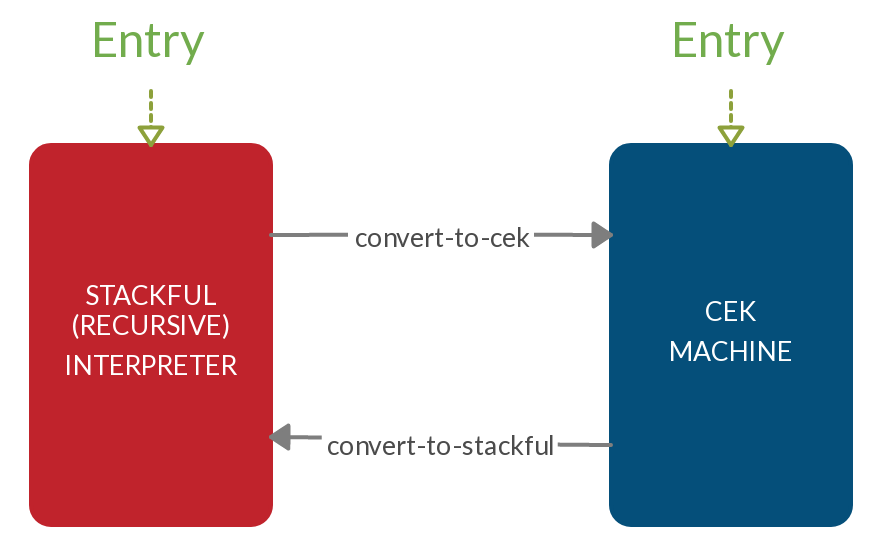
\includegraphics[scale=0.15]{img/cek-stackful-switch}
  \caption[hede]{Stackful \& CEK Switch}
  \label{fig:cek--switch-stack}
  \end{mdframed}
%\end{figure}
\end{wrapfigure}


To address this issue (without modifying the underlying framework nor
the GC), we propose to use a stackful interpreter to decrease the
continuation allocations on the heap. The stackful interpreter here is
a simple recursive interpreter for evaluating Racket forms, which is
translated by the RPython framework into a recursive C program that
uses the native stack. Recall that, however, the Pycket's interpreter
is based on the CEK machine, and the heap allocated explicit
continuations makes it very convenient to implement complex control
operations with continuations (as well as the proper handling of
tail-calls). Therefore the proposed approach is to use a stackful
interpreter \emph{alongside} the CEK, rather than replacing the
current CEK with a stackful interpreter. The idea is to use the stack
and heap in balance to decrease the GC pressure and take advantage of
using the stack, such as rapid allocations, locality etc.

Using the stack to implement a language like Racket, however,
understandibly introduces some challenges regarding the stack
management, such as handling overflows due to arbitrarily deep
recursion. Additionally, implementing a stackful interpreter on Pyket
for the entire Racket would be illogical, since it would not only
require implementing everything from scratch including the
continuations, but also not benefit from the current CEK's
performance. Therefore the logical approach is to use the two
interpreters together, repeatedly switch between the two whenever
appropriate, making sure that the switches don't induce a high
performance overhead.

One of the most fundamental points here is the interaction between the
two interpreters. Essentially, we want to use the stack to save some
heap space (thereby reducing the GC pressure) and take advantage of
faster allocations and locality. On the other hand, we don't want to
lose the benefits of the JIT's performance optimizations on the
CEK. Moreover, the stack management needs to be on point to avoid
problems such as switching back to the CEK when the stack is very deep
(e.g. stack overflow), since that would require allocating enough
continuations on the heap to counterbalance the performance benefit we
get from using the stackful interpreter.

\begin{wrapfigure}[11]{r}{0.45\textwidth}
  \vspace{-0.6cm}
  \footnotesize
%\begin{figure}[h!]
  \begin{mdframed}
    \begin{align*}
      e &::=\; x\; |\; v\; |\; (e\; e\; \ldots)\; |\; (\textbf{if}\; e\; e\; e)\; |\; (o\; e\; e)\; \\
      \; &|\; (\textbf{begin}\; e\; e\; \ldots)\; |\; (\textbf{lambda}\; (x_{\_!\_}\; \ldots)\; e)\\
      \; &|\; (\textbf{set!}\; x\; e)\; |\; (\textbf{raises}\; e)\\
      \; &|\; (\textbf{let\dash values}\; (((x)\; e)\; \ldots)\; e)\\
      \; &|\; (\textbf{convert\dash to\dash stackful}\; e)\\
      \; &|\; (\textbf{convert\dash to\dash cek}\; e)
    \end{align*}
  \caption[hede]{Source Language for Stackful \& CEK Models}
  \label{fig:st-cek--source}
  \end{mdframed}
%\end{figure}
\end{wrapfigure}

To understand this problem better and to work on a simpler setup, I
developed a formalism that includes both the CEK machine and the
stackful interpreter, evaluating a very simple subset of Racket
together, shown in \figref{fig:st-cek--source}, which is similar to the
Racket Core language used in \secref{subsec:linklets-semantics} minus
the forms for the linklet variables, plus some \racketcode{convert}
forms for controlling the interpreter switches from the source
level. \figref{fig:cek--switch-stack} shows the overview of the
interaction between the two models. We can start with either of the
interpreters and switch back and forth between them using the
\racketcode{convert} forms manually within the source code.

\begin{minted}[numbersep=0pt,gobble=0,linenos,numbers=left,fontsize=\footnotesize,frame=lines]{racket}
(eval-stackful (let-values (((a) 3)) (convert-to-cek (let-values (((b) 1)) (+ a b)))))
(eval-cek (let-values (((a) 3)) (begin (convert-to-stackful (set! a 5)) a)))
\end{minted}

In addition the formalism, in order to see how well this would perform
in action, we also prototyped an implementation on Pycket. It works in
a similar way to the model in \figref{fig:cek--switch-stack}, except
the starting point is the CEK, because Pycket needs to instantiate and
import the bootstrapping linklets at the startup and start a
computation by loading and running the program via the
\racketcode{read}, \racketcode{expand} etc.

The CEK starts the computation and handles the control to the stackful
whenever it encounters a \racketcode{let} or a \racketcode{begin}
form. The switch happens by just calling the stackful interpreter. The
stackful interpreter includes a trampoline to handle the tail-calls,
and in the current implementation it automatically switches back to
the CEK whenever \textbf{i)} it returns, or \textbf{ii)} a CPSed
primitive (e.g. a higher order function) is used, or \textbf{iii)} a
stack overflow is detected. The switch back to the CEK happens by
rewinding the stack via a \verb|ConvertStack| exception in which the
forms in each activation record installs a continuation. The CEK takes
the control and all the information at the previous switch-to-stack
point and continues from there.

\begin{wrapfigure}[19]{r}{0.5\textwidth}
  \vspace{-0.7cm}
\small
\begin{lstlisting}[mathescape]
(define (branchy lst)
  (letrec
    ([loop
      (lambda (lst)
        (let ([index (if (null? lst) 3 (car lst))])
          (if (null? lst)
              -1
              (if (< index 3)
                  (if (< index 2)
                      (loop (cdr lst))
                      (+ 3 (loop (cdr lst))))
                  (if (< index 5)
                      (if (< index 4)
                          (loop (cdr lst))
                          (+ 5 (loop (cdr lst))))
                      (if (< index 6)
                          (loop (cdr lst))
                          (+ 1 (loop (cdr lst)))))))))])
   (loop lst)))
\end{lstlisting}
\caption{A simple program with non-trivial control flow.}
\label{fig:branchy}
\end{wrapfigure}

The main investigation here is about the increase in the overall
performance with the following constraints: \textbf{i)} The number of
points where a switch occurs between the two interpreters and the
switching overhead should both be minimal, and \textbf{ii)} the amount
of copying activation records from the stack into the continuations in
the heap should be bounded. Since we're interested in the performance
on self-hosting Racket on Pycket, we are still interested in
interpreter-style dispatch loops. Therefore as a preliminary
experiment, we synthesized a program by simplifying the Racket's
\racketcode{fasl->s-exp} function from the FASL\footnote{fast-load
  serialization} library, which deserializes a given byte stream into
an s-expression. \figref{fig:branchy} shows the simplified program,
which takes a list of numbers and takes different branches depending
on the number. Note that some of the recursive calls are not
tail-calls, i.e. installs a continuation every time it is evaluated.

We ran this program on Pycket using Stackful+CEK and only-CEK with
different auto-generated inputs containing; only 1s, only 2s, and
random [0-7], each having 1000 and 2000 numbers. The runtimes for the
ones with only 1s and 2s are quite similar, except a larger warmup
time for the stackful interpreter, which is expected since RPython's
meta-tracing is not designed for recursive interpreters, therefore it
needs to be further optimized. However, we observe a consistent
increase in the run-time performance in the randomized experiments
(both 1000 and 2000) which visits different branches. Below are the
medians for the run-times for the experiments using 1000 numbers.
\vspace{-0.3cm}
\begin{figure}[h]
%\begin{wrapfigure}{l}{0.5\textwidth}
  \centering
  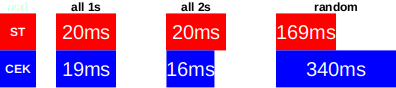
\includegraphics[scale=0.5]{img/stackful2}
\end{figure}
%\end{wrapfigure}

\vspace{-0.2cm}

Because of the limitations in the variety of programs that the
stackful interpreter can currently run (without large amounts of
switching), I seek to further characterize the performance of the
stackful evaluation along the CEK interpreter especially on programs
with heavy use of continuations.

Taking a step towards solving the fundamental issues in self-hosting
on meta-tracing, namely, intelligent meta-tracing of the programs with
complex control-flow and proper handling of the heap pressure, will
allow efficient self-hosting of Racket on meta-tracing Pycket. We
believe these are broadly applicable solutions that will serve as
principle approaches in self-hosting on meta-tracing frameworks in
general.
